\documentclass{beamer}

\useoutertheme[glossy]{wuerzburg}
\useinnertheme[shadow,outline]{chamfered}
\usecolortheme{shark}
\beamertemplatenavigationsymbolsempty 

\usefonttheme{professionalfonts}
\let\digamma\relax
\usepackage[scale=0.85,stdmathitalics=true,romanfamily=casual]{lucimatx}
\usefonttheme[stillsansseriftext]{serif}


\usepackage{fancyvrb}

%% Fancy syntax coloring via pygments
\usepackage{minted}
\definecolor{bg}{rgb}{0.95,0.95,0.95}
\usemintedstyle{borland}


\newenvironment{Rcode}
{\VerbatimEnvironment
 \begin{minted}[fontsize=\scriptsize,baselinestretch=1]{r}}%
{\end{minted}}

\newenvironment{Pcode}
{\VerbatimEnvironment
 \begin{minted}[fontsize=\scriptsize,baselinestretch=1]{python}}%
{\end{minted}}

\newenvironment{Code}[1]
{\VerbatimEnvironment
 \begin{minted}[fontsize=\scriptsize,baselinestretch=1]{#1}}%
{\end{minted}}


\usepackage{textfit} % commands \scaletoheight{height}{text} and \scaletowidth{width}{text}

\usepackage{tikz}


\newtheorem{Alert}{Alert}
\newtheorem{Highlight}{Highlight}

\newcommand{\Species}[1]{{\rmfamily \itshape #1}}
\newcommand{\Real}{\ensuremath{\mathbb{R}}}
\newcommand{\RealN}{\ensuremath{\mathbb{R}^n}}
\newcommand{\RealP}{\ensuremath{\mathbb{R}^p}}
\newcommand{\Mtx}[1]{\ensuremath{\mathbf{#1}}}
\newcommand{\Inv}[1]{\ensuremath{#1^{-1}}}
\newcommand{\InvMtx}[1]{\ensuremath{\mathbf{#1}^{-1}}}
\newcommand{\Red}[1]{\textcolor{red}{#1}}
\newcommand{\PsInv}[1]{\ensuremath{\mathbf{#1}^{+}}}



\usepackage{pdfpages}

\parskip=0.5em

%===========================================================
% Title Info
\title{Scientific Computing for Biologists}
\subtitle{Lecture 10: K-Means Clustering and Mixture Models} % (optional)

\author{Instructor: Paul M. Magwene}
\date{08 November 2011}


\begin{document}

\begin{frame}
\titlepage
\end{frame}



%===========================================================
\begin{frame}
  \frametitle{Outline of Lecture}

\begin{itemize}
    \item K-means clustering    
    \item Mixture model based clustering
\end{itemize}    

\end{frame}



%===========================================================
%% K-means clustering

\begin{frame}
\frametitle{K-mean Clustering}

\begin{block}{General idea}
Assign the $n$ data points (or $p$ variables) to one of $K$ clusters to as to optimize some criterion of interest.    
\end{block}

\begin{columns}
    
\begin{column}{5cm}
\begin{itemize}
\item The most common criterion to minimize is the sum-of-squares from the group centroids.

\[
V = \sum_{i=1}^k \sum_{j \in g_i}|x_j-\mu_i|^2
\]
\end{itemize}
\end{column}

\begin{column}{5.5cm}
\begin{center}
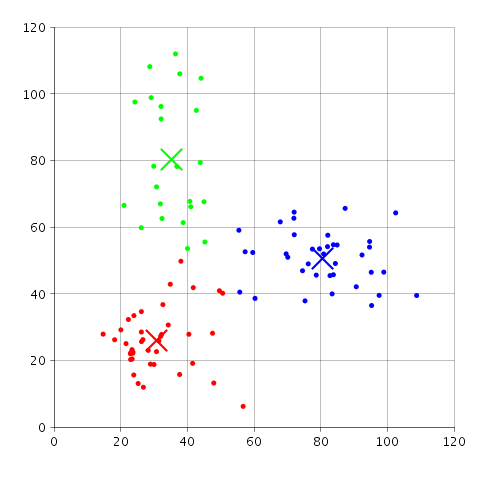
\includegraphics[width=0.9\textwidth]{k-means-simple.png}    
\end{center}
\end{column}

\end{columns}


\end{frame}
%===========================================================

%===========================================================
\begin{frame}
\frametitle{Simple algorithm for K-means clustering}
\begin{enumerate}
\item Decide on $k$, the number of groups

\item Randomly pick $k$ of the objects to act as the initial centers

\item Assign each object to the group whose center it is closest to

\item Recalculate the $k$ centers as the centroids of the objects assigned to them

\item Repeat from step 3 until centroids no longer move (convergence)

\end{enumerate}
\end{frame}
%===========================================================

%===========================================================
\begin{frame}
\frametitle{Illustration of K-means algorithm}
\begin{center}
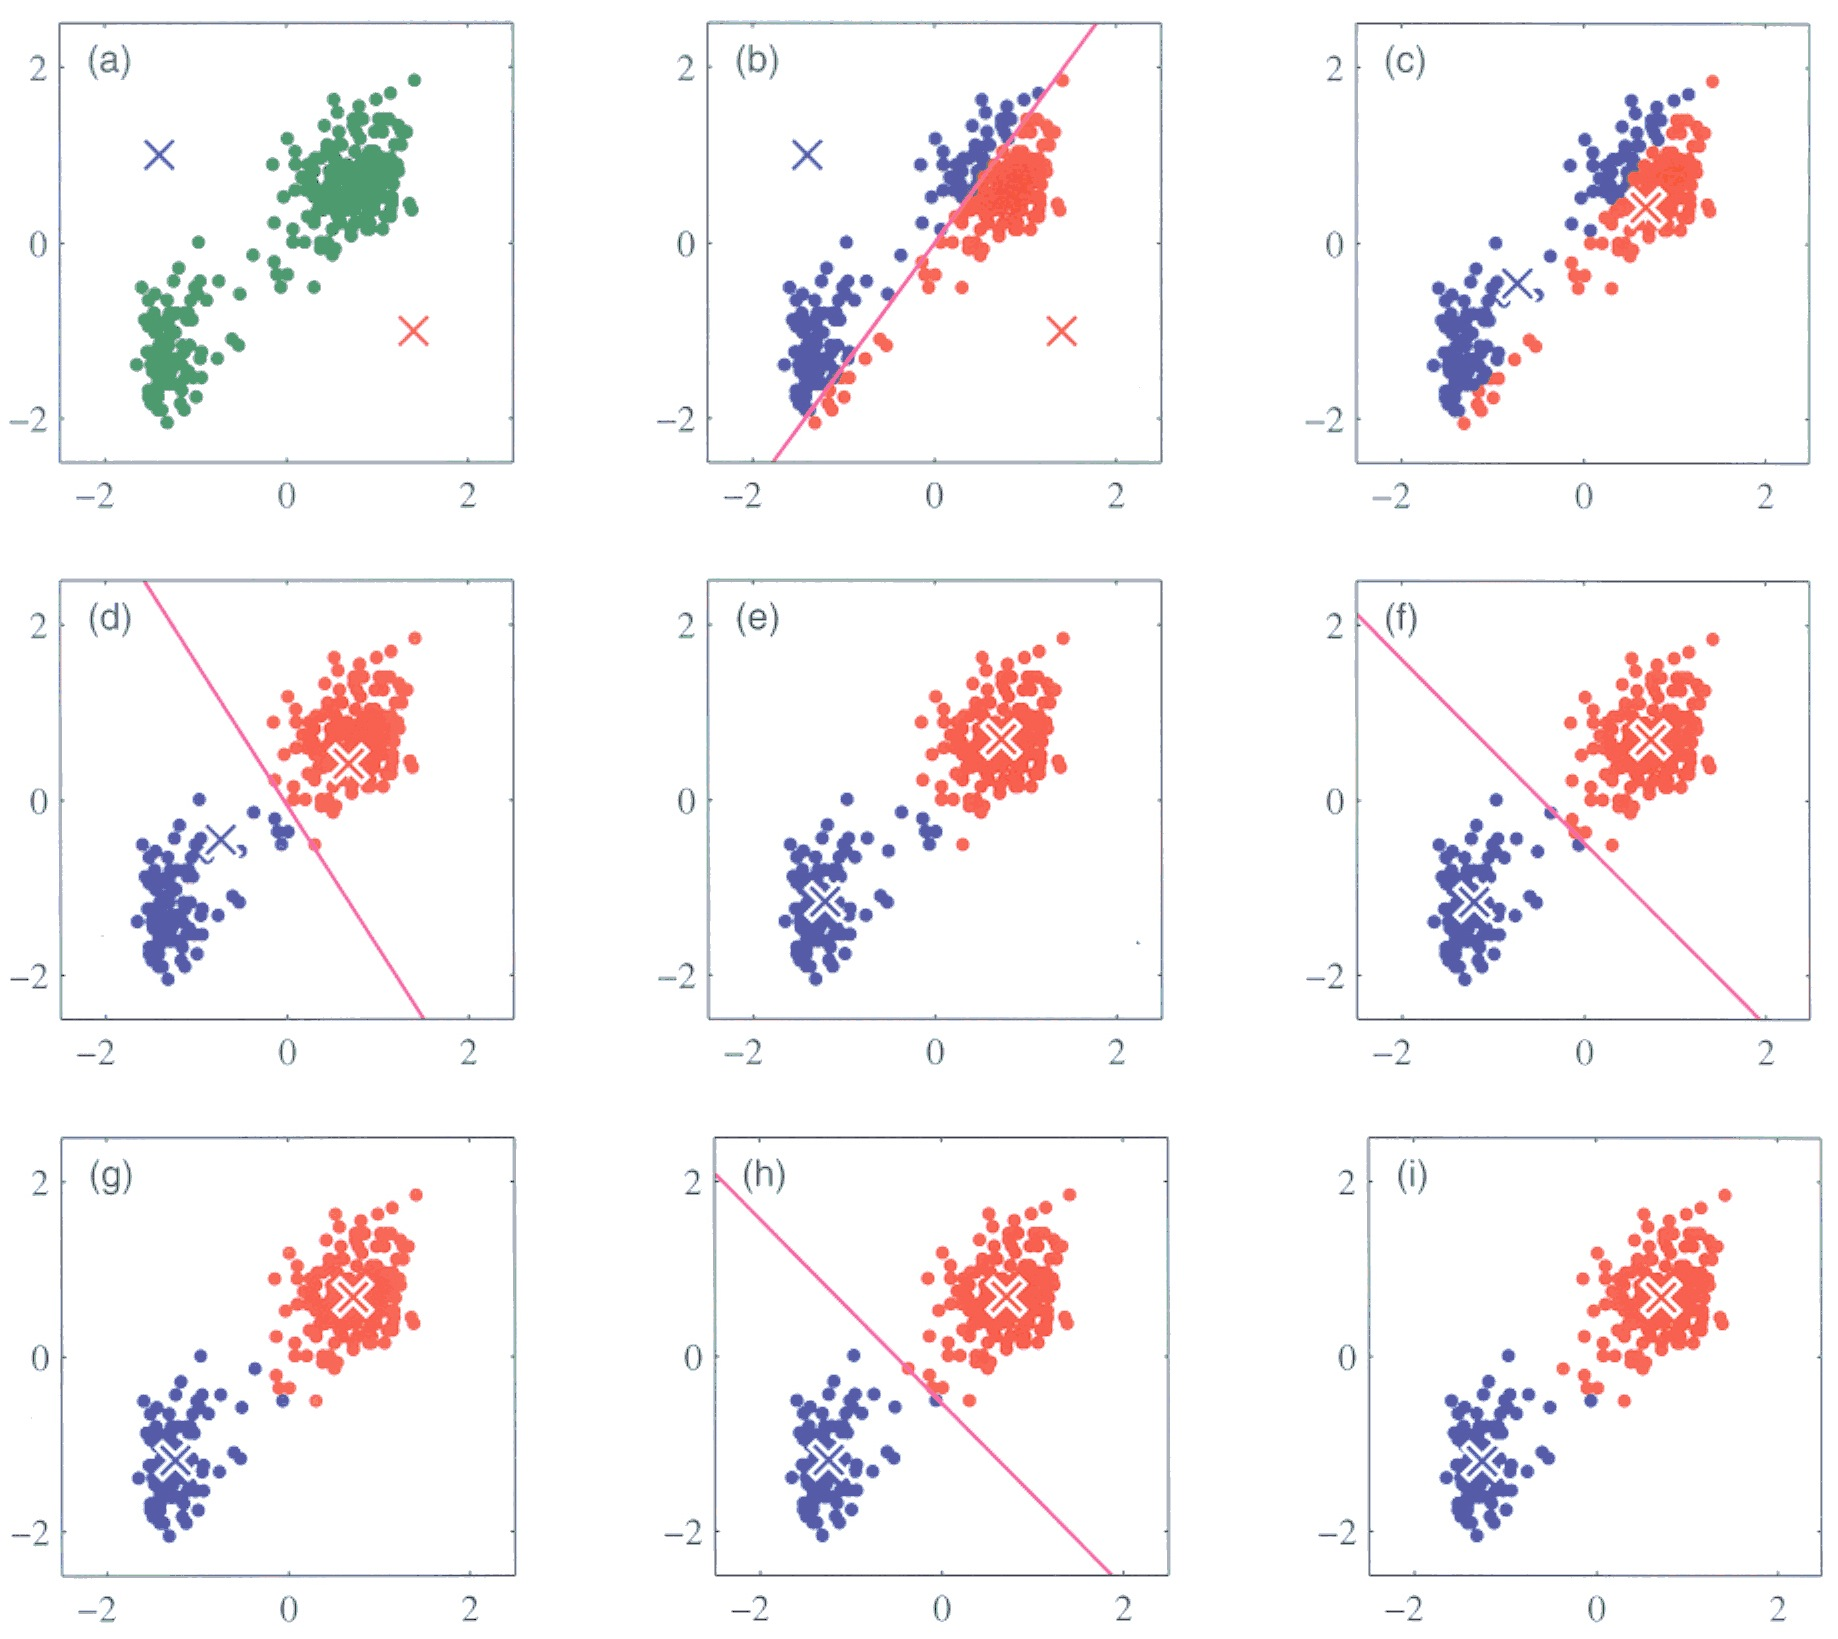
\includegraphics[height=3.2in]{k-means-fig.jpg}    
\end{center}
\end{frame}
%===========================================================

%===========================================================
\begin{frame}
\frametitle{Things to note re:K-means clustering}
\begin{itemize}
\item The algorithm described above does not necessarily find the global optimum

\bigskip

\item The algorithm is sensitive to choice of initial cluster center; k-means is often run multiple-time with different initial centers to insure inferred clusters are robust.    
\end{itemize}
\end{frame}
%===========================================================

%===========================================================
\begin{frame}
  \frametitle{Clustering with Mixture Models}

\begin{block}{Goal}
Method for assigning observations to clusters and estimating parametric distributions that describe the clusters.
\end{block}

    Assume that the data set represents observations drawn from a mixture of $g$ sub-distributions (user specifies $g$), and that the probability density function of the mixture is given by:
    
\[
p_{\mathrm{mix}} = \sum_{s=1}^g \pi_s p(\Mtx{x};\Mtx{\theta}_s)
\]

Where the $p(\Mtx{x};\Mtx{\theta}_s)$ represents the $s$-th `component density' (sub-distributions) and the $\Mtx{\theta}_s$ are the component parameters.  The $\pi_s$ represent the weighting factor of the $s$-th component in the mixture.

\end{frame}
%===========================================================

%===========================================================
% Pull in slides from PDF
{ 
\setbeamercolor{background canvas}{bg=} 
\includepdf[pages=14]{li-mixtures-lecture.pdf}
}
%===========================================================

%===========================================================
\begin{frame}
  \frametitle{Gaussian Mixture Models}

A common starting point in mixture modeling is to assume that the components are Gaussian.

If the data are univariate, then the mixture model is given by:

\[
p_{\mathrm{mix}} = \sum_{s=1}^g \pi_s f(\Mtx{x}|\mu_i, \sigma_i^2)
\]

where the $\mu_i$ and $\sigma_i$ are the means and standard deviations of each component distribution and:

\[
f(\Mtx{x}|\mu, \sigma) = \frac{1}{\sqrt{2\pi\sigma^2}}e^{-\frac{(x-\mu)^2}{2\sigma^2}}
\]

\end{frame}

%===========================================================


%===========================================================
\begin{frame}
  \frametitle{Example: Waiting time between Old Faithful eruptions}

\begin{center}
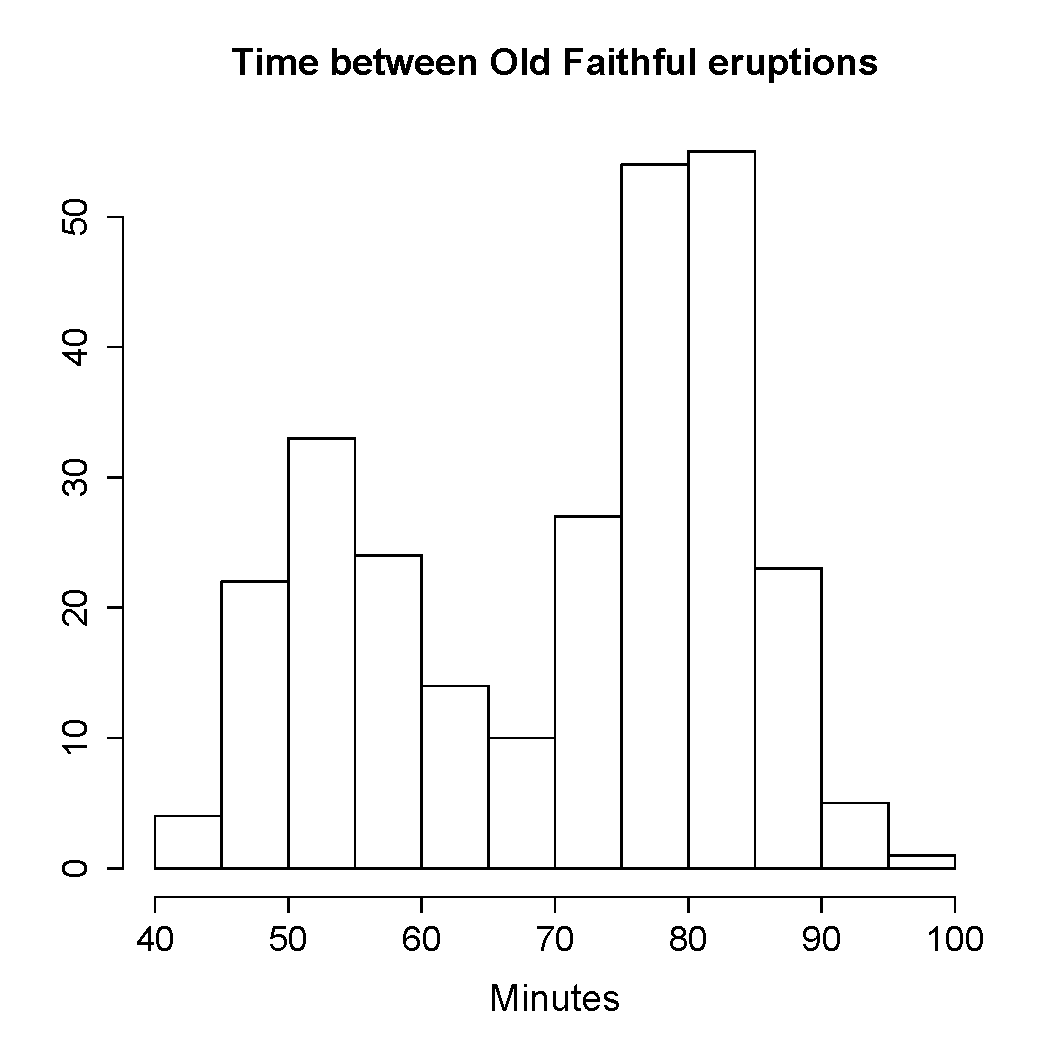
\includegraphics[height=3.1in]{waitingtime.pdf}    
\end{center}

\end{frame}
%===========================================================

%===========================================================
\begin{frame}
  \frametitle{Example: Gaussian fit, Old Faithful waiting time}

\vspace*{-0.15in}
\begin{columns}
\begin{column}{7cm}
\begin{center}
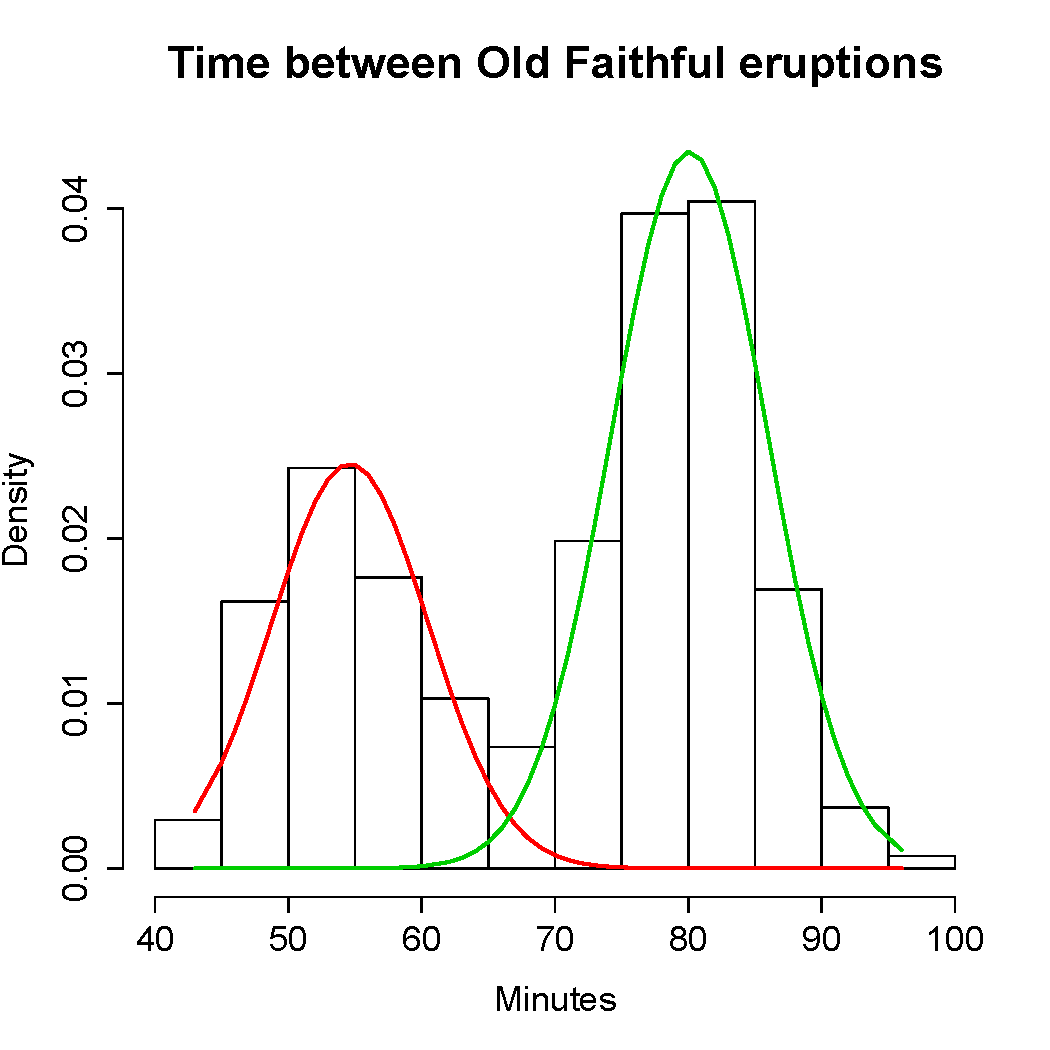
\includegraphics[height=3in]{waiting-fit.pdf}  
\end{center}
\end{column}


\begin{column}{5cm}
\begin{eqnarray*}
\pi = (0.36, 0.64)\\
\mu = (54.6, 80.1)\\
\sigma = (5.87, 5.87) 
\end{eqnarray*}
\end{column}

\end{columns}



\end{frame}
%===========================================================





%===========================================================
\begin{frame}
  \frametitle{Gaussian Mixture Models, Multivariate data}

When the components are multivariate Gaussian distributions:

\[
N(\Mtx{x};\Mtx{\theta}) \equiv (2\pi)^{-D/2}|\Sigma|^{-1/2} \exp 
\left[
-\frac{1}{2}(\Mtx{x}-\Mtx{\mu})^{T} \Sigma^{-1} - (\Mtx{x}-\Mtx{\mu})
\right]
\]

each with a different mean vector, $\Mtx{\mu}$ ($\Mtx{\mu} \in \Real^p$), and covariance matrix, $\Sigma$ ($p \times p$).

\end{frame}
%===========================================================

%===========================================================
\begin{frame}
\frametitle{Mixture Model Clustering, Example}
\begin{center}
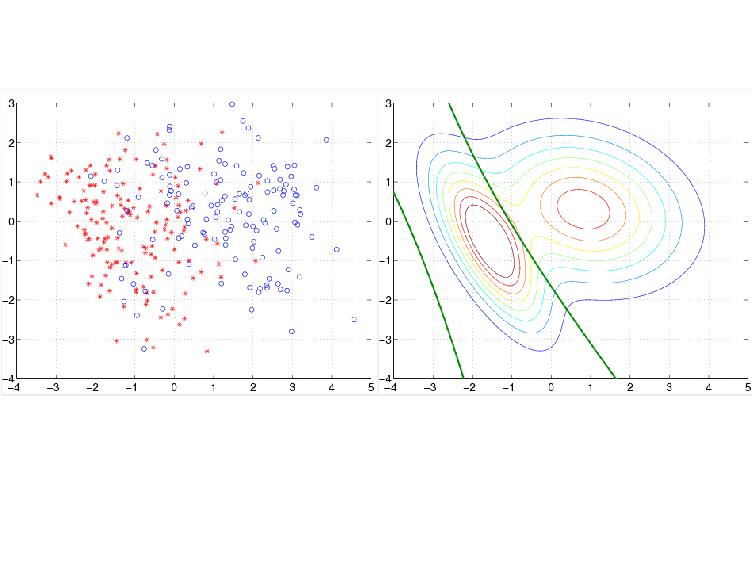
\includegraphics[width=\textwidth]{heart-disease.pdf}    
\end{center}

Heart disease example: 297 samples (137 with heart disease). 13 quantitative varibles (e.g. cholesterol, max heart rate, etc). Data centered and normalized. Data projected onto first two PCs. Two-component Gaussian mixture fit.

\end{frame}
%===========================================================


%===========================================================
\begin{frame}
  \frametitle{How do we `solve' the mixture model problem?}

The mixture model problem involves optimization over multiple parameters.

The standard approach to estimating the parameters is called the "Expectation-Maximization" (EM) algorithm.

\begin{itemize}
    \item Described by Dempster, Laird, and Rubin (1977)
    \item Provides a way to iterative compute a maximum likelihood estimation when the observed data are incomplete or there are `latent' parameters.
\end{itemize}


\end{frame}
%===========================================================

%===========================================================
\begin{frame}
  \frametitle{Overview of the EM Algorithm}

\begin{enumerate}
    \item Guess a set of starting parameters 
    \item Use these starting parameters to `estimate' the complete data
    \item Use the estimates of the complete data to update the parameters
    \item Repeat steps 2 and 3 until convergence
\end{enumerate}

\end{frame}
%===========================================================



%===========================================================
% Pull in slides from PDF
{ 
\setbeamercolor{background canvas}{bg=} 
\includepdf[pages=24]{li-mixtures-lecture.pdf}
}
%===========================================================



\end{document}



%===========================================================
\begin{frame}
  \frametitle{XXX}

\end{frame}
%===========================================================

